\section{Варіаційна нерівність}

Розглянемо абстрактний (тобто поки що не накладаємо на нього ніяких обмежень і не вимагаємо від нього ніяких властивостей) оператор $A$ який діє на підмножині $C$ гільбертового простору $H$. 

\begin{definition}[варіаційної нерівності]
    Кажуть, що для точки $x \in C$ виконується \emph{варіаційна нерівність} якщо
    \begin{equation}
        \sp{A(x), y - x} \ge 0, \quad \forall y \in C.
    \end{equation}
\end{definition}

\begin{proposition}
    У випадку $C = H$ виконання варіаційної нерівності для точки $x$ рівносильне виконанню рівності $A(x) = 0$.
\end{proposition}

\begin{proof}
    Справді, у випадку $C = H$ точка $y$ пробігає увесь простір $H$. Тому для довільної фіксованої точки $x$ точка $y - x$ також пробігає увесь простір $H$. Візьмемо $y$ такий, що $y - x = -A(x)$, тоді 
    \begin{equation}
        \sp{A(x), y - x} = \sp{A(x), -A(x)} = - \no{A(x)}^2 \le 0,
    \end{equation}
    причому рівність можлива лише якщо $A(x) = 0$. Отже, варіаційна нерівність може виконуватися тоді і тільки тоді, коли $A(x) = 0$.
\end{proof}

\section{Зв'язок із задачами оптимізації}

Прояснимо зв'язок варіаційної нерівності із задачами оптимізації. \medskip

\begin{proposition}
    Для задачі
    \begin{equation}
        f \to \Min_C
    \end{equation}
    у випадку опуклості як $f$ так і $C$ критерієм того, що точка $x$ є розв'язком є виконання нерівності
    \begin{equation}
        \sp{f'(x), y - x} \ge 0, \quad \forall y \in C.
    \end{equation}
\end{proposition}

\begin{proof}
    Запишемо лінійну апроксимацію $f$: 
    \begin{equation}
        f(y) = f(x) + \sp{f'(x), y - x} + o \left( \no{y - x} \right).
    \end{equation}
    
    Припустимо тепер, що другий доданок менше нуля для якогось $y = x + z$, тоді
    \begin{equation}
        f(x + z) - f(x) = \sp{f'(x), z} + o \left( \no{z} \right).
    \end{equation}

    Розглянемо (з опуклості $C$ випливає, що $x + \epsilon z \in C$, а отже можемо підставляти таке $y$) тепер $y = x + \epsilon z$, отримаємо
    \begin{equation}
        f(x + \epsilon z) - f(x) = \sp{f'(x), \epsilon z} + o \left( \no{\epsilon z} \right).
    \end{equation}

    З визначення $o(\cdot)$ зрозуміло, що при $\epsilon \to +0$ знак правої частини визначає перший доданок. \medskip
    
    Тобто, права частина буде від'ємоною для якогось достатньо малого $\epsilon$. Але тоді від'ємною буде і ліва частина, $f(x + \epsilon z) - f(x) < 0$. Але це означає, що $f(x + \epsilon z) < f(x)$. Отже, $x$ не є точкою мінімуму $f$ на $C$. Отримане протиріччя завершує доведення.
\end{proof}

\begin{remark}
    У випадку відсутності опуклості або $f$ або $C$ або і того і того, цей критерій перетворюється на необхідну умову.
\end{remark}

% \begin{example}
%     TODO: навести контрприклади.
% \end{example}

\section{Зв'язок із сідловими точками}

Розглянемо тепер оптимізацію з обмеженнями, тобто задачу
\begin{equation}
    f(x) \xrightarrow[\substack{g_i(x) \le 0 \\ i = 1 \ldots n}]{} \min.
\end{equation}

Для цієї задачі можна побудувати функцію Лагранжа,
\begin{equation}
    L (x, y) = f + \Sum_{i = 1}^n y_i g_i(x),
\end{equation}
де $y_i$ --- множники Лагранжа. \medskip
% , які зазвичай позначаються $Lmbda_i$.

Постає задача пошуку сідлової точки (справді, якщо у $f$ мінімум в $\bar x$, то у $L$ в $(\bar x, \bar y)$ буде мінімум по $x$ і максимум по $y$, і навпаки) функції $L$. 

\begin{definition}[сідлової точки]
    Точка $(\bar x, \bar y)$ називається \emph{сідловою точкою} функції $L$ якщо
    \begin{equation}
        L(\bar x, y) \le L(\bar x, \bar y) \le L(x, \bar y) \quad \forall x \; \forall y
    \end{equation}
    тобто по $x$ маємо мінімум в $\bar x$, а по $y$ --- максимум в $\bar y$.
\end{definition}

Можемо записати ці умови наступним чином:
\begin{equation}
    \left\{
        \begin{aligned}
            & \sp{\nabla_1 L(\bar x, \bar y), x - \bar x} \ge 0 \quad \forall x \in C_1 \subseteq H_1, \\
            & \sp{-\nabla_2 L(\bar x, \bar y), y - \bar y} \ge 0 \quad \forall y \in C_2 \subseteq H_2,
        \end{aligned}
    \right. 
\end{equation}

\begin{remark}
    Ці нерівності можна об'єднати в одну:
    \begin{equation}
        \sp{\nabla_1 L(\bar x, y), x - \bar x} + \sp{-\nabla_2 L(\bar x, \bar y), y - \bar y} \ge 0.
    \end{equation}
\end{remark}

\section{Ерроу та Гурвіц}

\begin{example}
    Розглянемо тепер цілком конкретну функцію $L(x, y) = x \cdot y$ і спробуємо знайти її сідлову точку.
\end{example}

\begin{solution}
    Розглянемо алгоритм
    \begin{equation}
        \begin{aligned}
            x_{k + 1} &\coloneqq x_k - \rho_k \nabla_1 L(x_k, y_k) = x_k - \rho_k y_k, \\
            y_{k + 1} &\coloneqq y_k + \rho_k \nabla_2 L(x_k, y_k) = y_k + \rho_k x_k,
        \end{aligned}
    \end{equation}
    який називається \textit{методом Ерроу-Гурвіца}. \medskip
    
    % \inputminted[linenos]{python}{src/arrow_hurwitz.py}

    Покладемо $(x_0, y_0) = (1, 1)$, $\rho_k \equiv 1$ і побачимо наступні ітерації:
    \begin{figure}[H]
        \centering
        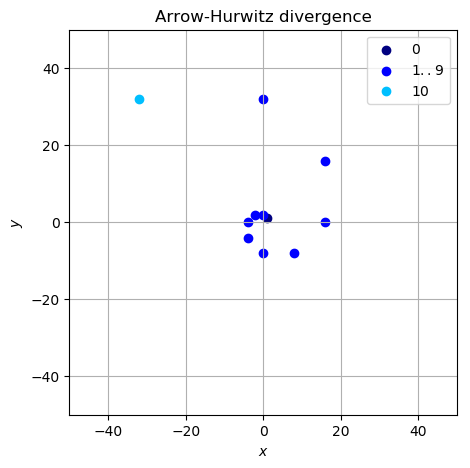
\includegraphics{img/arrow-hurwitz-divergence.png}
    \end{figure}

    Вони, очевидно, розбігаються, хоча здавалося що ми рухаємося у напрямку правильних градєнтів по кожній з компонент.

    \begin{remark}
        Для цієї задачі змінний розмір кроку нас не врятує, його зменшення тільки згладить спіраль по якій точки розбігаються.
    \end{remark}

    Окрім емпіричних спостережень, ми можемо явно довести розбіжність, розглянемо для цього $|x_{k+1}|^2 + |y_{k+1}|^2$:
    \begin{multline}
        |x_{k+1}|^2 + |y_{k+1}|^2 = |x_k - \rho_k y_k|^2 + |y_k + \rho_k x_k|^2 = \\
        = |x_k|^2 + \rho_k^2 \left( |x_k|^2 + |y_k|^2 \right) + |y_k|^2 > |x_k|^2 + |y_k|^2,
    \end{multline}
    у той час як сідловою точкою, очевидно, є $(0, 0)$.
\end{solution}

\begin{remark}
    Не зважаючи на розбіжність методу Ерроу-Гурвіца на такій простій задачі, Ерроу свого часу був удостоєний Нобелівськиї премії з економіки, за задачі які цим методом можна розв'язати.
\end{remark}

Виникає закономірне зпитання а що ж це за задачі такі. 

\section{Сильно опуклі функції}

Для відповіді на це питання нам доведеться ввести 

\begin{definition}[сильно опуклої функції]
    Функція $f = f(x)$ називається \emph{$\mu$-сильно опуклою} для деякого $\mu > 0$ якщо
    \begin{equation}
        f(\alpha \cdot x + (1 - \alpha) \cdot y) \le \alpha \cdot f(x) + (1 - \alpha) \cdot f(y) - \mu \cdot \alpha \cdot (1 - \alpha) \cdot \no{x - y}^2.
    \end{equation}
\end{definition}

Про всяк введемо також трохи більш узагальнене

\begin{definition}[сильно опуклої функції]
    Функція $f = f(x)$ називається \emph{$g$-сильно опуклою} для деякої $g$ якщо
    \begin{equation}
        f(\alpha \cdot x + (1 - \alpha) \cdot y) \le \alpha \cdot f(x) + (1 - \alpha) \cdot f(y) - \alpha \cdot (1 - \alpha) \cdot g(\no{x - y}).
    \end{equation}
\end{definition}

Можемо записати також альтернетивне визначення
% (чи то пак критерій\todo{Довести, що це критерій.}) 
$\mu$-сильно опуклості:
\begin{equation}
    f(y) \ge f(x) + \sp{\nabla f(x), y - x} + \mu \cdot \no{x - y}^2.
\end{equation}

Так от виявляється, що для задач із сильно опуклою функцією $f$ метод Ерроу-Гурвіца збігається. Доведення наводиться нижче у більш загальному випадку, а поки що останннє
\begin{remark}
    Існують певні ергодичні теореми, які стверджують збіжність середнього значення 
    \begin{equation}
        \left(\tilde x_n, \tilde y_n\right) = \left( \frac{x_0 + \ldots + x_n}{n + 1}, \frac{y_0 + \ldots + y_n}{n + 1} \right)
    \end{equation}
    до якоїсь сідлової точки $(\bar x, \bar y)$, але подібні усереднені методи не є практичними, адже вони збігаються дуже повільно, а у задачі вище вже за тисячу ітерацій числа стають настільки великі що машинні похибки ``переважають'' усю теорію.
\end{remark}

\section{Монотонні оператори}

Нагадаємо, що ми намгаємося знайти точку $x \in C$ яка задовольняє варіаційній нерівності
\begin{equation}
    \sp{A x, y - x} \ge 0 \quad \forall y \in C,
\end{equation}
де оператор $A$, взагалі кажучи, не нерозтягуючий. \medskip

Подивимося
% \todo{Показати еквівалентність.}
на цю задачу як на задачу знаходження нерухомої точки оператора
\begin{equation}
    T: x \mapsto P_C \left( x - \rho A x \right),
\end{equation}
де $\rho > 0$. Одразу зауважимо, що ці міркування приводять нас до наступного алгоритму
\begin{equation}
    x_{k + 1} \coloneqq P_C \left( x_k - \rho_k A x_k \right),
\end{equation} 
збіжність якого ми зараз і проаналізуємо. \medskip

Взагалі хотілося б (відомо багато теорем щодо збіжності описаного алгоритму за таких умов) щоб оператор $T$ був нерозтягуючим. Маємо:
\begin{multline}
    \no{T x - T y}^2 \le \no{x - y - \rho (A x - A y)}^2 \le \\
    \le \no{x - y}^2 - 2 \rho \sp{A x - A y, x - y} + \rho^2 \no{A x - Ay}^2.
\end{multline}

Для подальших оцінок нам знадобиться поняття монотонного оператора.

\begin{definition}[монотонного оператора]
    Оператор $A$: $H \to H$ називається \emph{монотонним} якщо
    \begin{equation}
        \sp{A x - A y, x - y} \ge 0 \quad \forall x \; \forall y.
    \end{equation}
\end{definition}

Поняття монотонності для операторів відіграє схожу роль з поняттям монотонності функцій.

\begin{example}
    Оператор $A$ називається \emph{опуклим} якщо його градієнт $\nabla A$ монотонний.
\end{example}

Аналогічно до $\mu$-сильно опуклих функцій існуюють $\mu$-сильно опуклі оператори, для визначення яких вводиться
\begin{definition}[сильно монотонного оператора]
    Оператор $A$: $H \to H$ називається \textit{$\mu$-сильно монотонним} зі сталою $\mu > 0$ якщо
    \begin{equation}
        \sp{A x - A y, x - y} \ge \mu \cdot \no{x - y}^2 \quad \forall x \; \forall y.
    \end{equation}
\end{definition}

Якщо оператор $A$ --- $\mu$-сильно монотонний то можемо продовжити ланцюжок оцінок:
\begin{multline}
    \no{x - y}^2 - 2 \rho \sp{A x - A y, x - y} + \rho^2 \no{A x - Ay}^2 \le \\
    \le \no{x - y}^2 - 2 \rho \mu \no{x - y}^2 + \rho^2 \no{A x - A y}^2.
\end{multline}

Якщо ж при цьому оператор $A$ ще й $L$-ліпшицеви (ліпшицевий з константою $L$, тобто $\no{A x - A y} \le L \cdot \no{x - y}$), то можемо продовжити ще:
\begin{multline}
    \no{x - y}^2 - 2 \rho \mu \no{x - y}^2 + \rho^2 \no{A x - A y}^2 \le \\
    \le \no{x - y}^2 - 2 \rho \mu \no{x - y}^2 + \rho^2 L^2 \no{x - y}^2 = \\
    = (1 - 2 \rho \mu + \rho^2 L^2) \no{x - y}^2 = \kappa(\rho) \cdot \no{x - y}^2.
\end{multline}

тобто достатньо обрати $\rho$ так, щоб $\kappa(\rho) \in (0, 1)$. \medskip

Розв'язуючи отриману квадратну нерівність знаходимо:
\begin{equation}
    \rho \in \left(0, \frac{2 \mu}{L^2}\right),
\end{equation}
тобто знайшли цілий інтервал значень $\rho$ для яких наш алгоритм буде збіжним. \medskip

Здавалося б все добре, але подивимося, у якій точці досягається мінімум $\kappa(\rho)$:
\begin{equation}
    \tilde \rho = \frac{\mu}{L^2},
\end{equation}
і чому він дорівнює:
\begin{equation}
    \kappa(\tilde \rho) = 1 - 2 \rho \mu + \rho^2 L^2 = 1 - 2 \frac{\mu}{L^2} \mu + \left( \frac{\mu}{L^2} \right)^2 L^2 = 1 - \frac{\mu^2}{L^2}.
\end{equation}

\begin{remark}
    На жаль, правда життя така, що $\mu$ зазвича доволі мале, а $L$ навпаки --- доволі велике, тому $\rho < 1$ але зовсім трохи. А це у свою чергу означає повільну збіжність.
\end{remark}

\section{Регуляризація}

У той же час майже довільну опуклу функцію $f$ можна замінити (цей процес називається регуляризацією) на $\epsilon$-сильно опуклу функцію $f_\epsilon = f + \epsilon\no{x}^2$, тому може здатися, що всі наші проблеми розв'язані. \medskip

Так, у загальному випадку для монотонного оператора $A$ можна розглянути оператор $A_\epsilon = A + \epsilon {\bf 1}$, де ${\bf 1}$, $x \mapsto x$ --- \emph{одиничний} (\emph{тотожний}) \emph{оператор}. Тоді можемо записати
\begin{equation}
    \sp{A_\epsilon x - A_\epsilon y, x - y} = \underset{\ge 0}{\underbrace{\sp{A x - A y, x - y}}} + \epsilon \cdot \no{x - y}^2 \ge \epsilon \cdot \no{x - y}^2,
\end{equation}
тобто оператор $A_\epsilon$ є $\epsilon$-сильно опуклим. \medskip

Це наштовхує на думки про побудову алгоритму з ітераціями вигляду
\begin{equation}
    x_{k + 1} \coloneqq P_C \left( x_k - \rho_k A_{\epsilon_k} x_k \right),
\end{equation}
але тоді постає ще ряд запитань, наприклад які умови мають задовольняти $\{\rho_k\}_{k = 1}^\infty$ і $\{\epsilon_k\}_{k = 1}^\infty$ для збіжності цього алгоритму. Поки що ці запитання лишаємо без відповіді.

\section{Зв'язок із мережевими іграми і рівновагою Неша}

\emph{Цей розділ взято з доповіді} \href{https://simons.berkeley.edu/talks/asu-ozdaglar-3-28-18}{[Asu \"Ozdaglar, 2018]}. \medskip

У багатьох соціальних та економіних задачах, рішення окремих індивідів (агентів) залежать лише від дій їхніх друзів, колег, однолітків чи суперників. Як приклади можна навести:
\begin{itemize}
    \item Поширення інновацій, стилю життя.
    \item Формування громадських думок і соціальне навчання.
    \item Суперництво між конкурентними фірмами.
    \item Забезпечення суспільних благ.
\end{itemize}

Такі взаємодії можна промоделювати мережевою грою, що означає виконання наступних припущень:
\begin{itemize}
    \item Агенти взаємодіють по ребрам мережі, представленої графом.
    \item Виграш кожного гравця залежить від його власних дій і від \emph{агрегованого} значення дій агентів у його околі.
\end{itemize}

Формальніше, модель мережевої гри наступна: $n$ агентів взаємодіють по мережі $G \in \RR^{n \times n}$:
\begin{equation}
    \begin{cases}
        G_{i,j} > 0 & \text{вплив }j\text{ на }i, \\
        G_{i,i} = 0 & \text{без петель}.
    \end{cases}
\end{equation}

У кожного агента $i$ є:
\begin{itemize}
    \item стретегія $x^i \in \mathcal{X}^i$, де $\mathcal{X}^i \subset \RR^n$ --- допустима множина стратегій ;
    \item цільова функція $J^i(x^i, z^i(x)): \RR^n \times \RR^n \to \RR$, де $z^i(x) \coloneqq \sum_{j = 1}^n G_{i,j} x^j$ --- агрегатор.
\end{itemize}

Кожен агент намагється навчитися обчислювати свою оптимальну відповідь:
\begin{equation}
    x_\text{br}^i(z^i) \coloneqq \Argmin_{x^i \in \mathcal{X}^i} J^i(x^i, z^i).
\end{equation}

Нагадаємо
\begin{definition}[рівноваги за Нешем]
    Множина стратегій $\{\bar x_i\}_{i = 1}^n$ називається \emph{рівновагою за Нешем} якщо для кожного гравця $i$, $\bar x^i \in \mathcal{X}^i$:
    \begin{equation}
        J^i \left( \bar x^i, \sum_{j = 1}^n G_{i,j} \bar x^j \right) \le J^i \left( x^i, \sum_{j = 1}^m G_{i,j} \bar x^i \right), \quad \forall x^i \in \mathcal{X}^i.
    \end{equation}
\end{definition}

Можна показати, що при виконанні наступних припущень:
\begin{itemize}
    \item $\mathcal{X}^i \subset \RR^n$ --- замкнені, опуклі та обмежені;
    \item $J^i(x^i, z^i(x))$ опукла по $x^i$, для кожного вектора доповнюючих стратегій $x^{-i} \in \mathcal{X}^{-i}$;
    \item $J^i(x^i, z^i) \in C^2$ по $x^i$ і $z^i$.
\end{itemize}
справджується наступне
\begin{proposition}
    $\bar x$ є рівновагою за Нешем $\iff$ $\bar x$ є розв'язком варіаційної нерівності із допустимою множиною $\mathcal{X}$ і функцією $F$ визначеними наступним чином:
    \begin{align}
        \mathcal{X} &\coloneqq \mathcal{X}^1 \times \dots \times \mathcal{X}^n; \\
        F(x) &\coloneqq [F^i(x)]_{i = 1}^n \coloneqq \begin{bmatrix}
            \nabla_{x^1} J^1(x^1, z^1(x)) \\
            \vdots \\
            \nabla_{x^n} J^n(x^n, z^n(x)) 
        \end{bmatrix}
    \end{align}
\end{proposition}

\begin{proposition}[Facchinei та Pang, 2003]
    Якщо окрім цього, якобіан гри $F$ строго монотонний, то рівновага за Нешем існує та єдина.
\end{proposition}

\section{Зв'язок із транспортними мережами}

\emph{Цей розділ взято з книги} А. В. Гасникова, <<Введение в математическое моделирование транспортных потоков>>. \medskip

Розглянемо один із підходів до моделювання і дослідження транспортних потоків, що базується на теорії конкурентної безкоаліційної рівноваги, яка дозволяє описати доволі адекватних механізм функціонування автомобільних вулично-дорожніх мереж (ВДМ). \medskip

Моделі, яки ми розглянемо, застосовуються для отримання прогнозних оцінок завантаженності елементів транспортної мережі. Подібні задачі цікаві, зокрема, тим, що є одним із інструкментів об'єктиної оцінки ефективності проектів з модифікації ВДМ з точки зору розвантаження найбільш завантажених і проблемних ділянок доріг.

\subsection{Моделювання транспортних потоків як задача прийняття рішень}

Для визначення обсягів завантаження ВДМ у першу чергу необхідно з'я\-су\-ва\-ти, чим керуються водії, обираючи той чи інший маршрут. Поведінкові принципи користувачів транспортної мережі були остаточно сформульовані Вардропом у [J. Wardrop, Some Theoretical Aspects of Road Traffic Research, 1952], де він наводить дві можливі ситуації:
\begin{enumerate}
    \item користувачі мережі незалежно один від одного обирають маршрути з мінімальними затратами; (user optimization)
    \item користувачі мережі обирають маршрути з мінімальними сумарними затратами. (system optimization)
\end{enumerate}

\begin{definition}
    Ці принципи називаються, відповідно, \emph{першим і другим принципами Вардропа}.
\end{definition}

Перший принцип Вардропа відповідає конкурентнії безколіаційній рівновазі (жоден окремий користувач не може знизити свої витрати відхилившись від свого поточного маршруту). Цей принцип передбачає ідеальну інформованість окремих користувачів про витрати на усіх шляхах (сьогодні це досягається за допомогою розумних навігаторів), а також відсутність суттєвого впливу на витрати на шляхах зі сторони одного конкретного користувача (не виконується для вантажних автомобілів а також аварійних ситуацій, але здебільшого виконується). Резюмуючи, перший принцип Вардропа сьогодні доволі точно описує поведінкові принципи користувачів ВДМ, а не є якоюсь надміру ідеалізованою абстракцією.

\subsection{Формалізація задачі}

Виходячи з наведених міркувань, побудуємо економіко-математичну моделі розподілу транспортних потоків у ВДМ. Транспортну мережу опишему у вигляді орієнтованого графу $G(V, E)$, де $V$ --- множина вершин (перехресть), $E$ --- множина орієнтованих дуг мережі (доріг між сусідніми перехрестями). \medskip

При дослідженні потокоформуючих факторів у множині вершин розглянемо дві підмножини. Перше, $S \subset V$, містить пункти, що породжують потоки; елементи множини $S$ (sources) назвемо джерелами/витоками. Друге, $D \subset V$, містить пункти, що поглинають потоки; елементи множини $D$ (destinations) назвемо стоками. Для задачі моделюванні трудових міграцій (для ранкових годин пік), джерелами будуть спальні райони міста, а стоками --- ділові райони міста (для вечірніх годин ситуація рівно протилежна). \medskip

Через $P_{s,d}$ будемо позначати множину шляхів з витоку $s$ у стік $d$. Окремі шляхи із витоку $s$ у стік $d$ будемо позначати  $p_{s,d}$, або просто $p$ якщо витік і стік несуттєві. Через $f_p$ позначимо потік на шляху $p$, через $c_p(F)$ --- маргинальні затрати на шляху $p$ якщо загальна матриця потоків на шляхах дорівнює $F$ (природніми прикладами колм затрати на одному шляху залежать від завантаженості інших є перехрестя головних і другорядних доріг, або ж паралельні дороги). Зрозуміло, що умова рівноваги має наступний вигляд:
\begin{equation}
    \label{eq:flow-network-equilibrium}
    \text{якщо } f_{p_{s,d}} > 0 \text{, то } c_p(F) = \min_{p' \in P_{s,d}} c_{p'}(F).
\end{equation}

Окрім цього, для кожної пари $(s,d)$ існує певний сталий (у випадку трудових міграцій) попит на транспорт, який будемо позначати $\rho_{s,d}$. Зрозуміло, що оптимальний рівноважний потік також має задовольняти наступним консервативним умовам:
\begin{equation}
    \sum_{p \in P(s, d)} f_p = \rho_{s, d}.
\end{equation}

\begin{proposition}
    За таких умов допустима множина транспортних потоків $\mathcal{F}$ володіє гарними властивостями, а саме вона замкнута, опукла, і непорожня.
\end{proposition}

\subsection{Зведення до варіаційної нерівності}

Якщо залежність транспортних витрати від обсягів завантаження ВДМ є монотонною і неперевною, то пошук рівноважних потоків може бути зведений до розв'язання варіаційної нерівності.

\begin{theorem}
    Потік $F^\star \in \mathcal{F}$ задовольняє умову рівноваги \eqref{eq:flow-network-equilibrium} тоді і лише тоді, коли він є розв'язком варіаційної нерівності
    \begin{equation}
        \langle C(F^\star), F - F^\star \rangle \ge 0, \quad \forall F \in \mathcal{F},
    \end{equation}
    де у матрицю $C$ зібрані маргинальні транспортні витрати на усіх шляхах.
\end{theorem}

\section{Подальші припущення}

Надалі будемо розв'язувати наступну задачу:
\begin{equation}
    \label{eq:variational-inequality}
    \text{знайти } x \in C: \quad \sp{A x, y - x} \ge 0, \quad \forall y \in C. 
\end{equation}

Також будемо вважати, що виконані наступні умови:
\begin{itemize}
    \item множина $C \subseteq H$ --- опукла і замкнена;
    \item оператор $A: H \to H$ --- монотонний і ліпшицевий (із константою $L$);
    \item множина розв'язків \eqref{eq:variational-inequality} непорожня.
\end{itemize}
